\documentclass[a4paper]{tufte-handout}

% ams
\usepackage{amssymb,amsmath}

\usepackage{ifxetex,ifluatex}
\usepackage{fixltx2e} % provides \textsubscript
\ifnum 0\ifxetex 1\fi\ifluatex 1\fi=0 % if pdftex
  \usepackage[T1]{fontenc}
  \usepackage[utf8]{inputenc}
\else % if luatex or xelatex
  \makeatletter
  \@ifpackageloaded{fontspec}{}{\usepackage{fontspec}}
  \makeatother
  \defaultfontfeatures{Ligatures=TeX,Scale=MatchLowercase}
  \makeatletter
  \@ifpackageloaded{soul}{
     \renewcommand\allcapsspacing[1]{{\addfontfeature{LetterSpace=15}#1}}
     \renewcommand\smallcapsspacing[1]{{\addfontfeature{LetterSpace=10}#1}}
   }{}
  \makeatother

\fi

% graphix
\usepackage{graphicx}
\setkeys{Gin}{width=\linewidth,totalheight=\textheight,keepaspectratio}

% booktabs
\usepackage{booktabs}

% url
\usepackage{url}

% hyperref
\usepackage{hyperref}

% units.
\usepackage{units}


\setcounter{secnumdepth}{-1}

% citations
\usepackage{natbib}
\bibliographystyle{plainnat}


% pandoc syntax highlighting
\usepackage{color}
\usepackage{fancyvrb}
\newcommand{\VerbBar}{|}
\newcommand{\VERB}{\Verb[commandchars=\\\{\}]}
\DefineVerbatimEnvironment{Highlighting}{Verbatim}{commandchars=\\\{\}}
% Add ',fontsize=\small' for more characters per line
\newenvironment{Shaded}{}{}
\newcommand{\AlertTok}[1]{\textcolor[rgb]{1.00,0.00,0.00}{\textbf{#1}}}
\newcommand{\AnnotationTok}[1]{\textcolor[rgb]{0.38,0.63,0.69}{\textbf{\textit{#1}}}}
\newcommand{\AttributeTok}[1]{\textcolor[rgb]{0.49,0.56,0.16}{#1}}
\newcommand{\BaseNTok}[1]{\textcolor[rgb]{0.25,0.63,0.44}{#1}}
\newcommand{\BuiltInTok}[1]{#1}
\newcommand{\CharTok}[1]{\textcolor[rgb]{0.25,0.44,0.63}{#1}}
\newcommand{\CommentTok}[1]{\textcolor[rgb]{0.38,0.63,0.69}{\textit{#1}}}
\newcommand{\CommentVarTok}[1]{\textcolor[rgb]{0.38,0.63,0.69}{\textbf{\textit{#1}}}}
\newcommand{\ConstantTok}[1]{\textcolor[rgb]{0.53,0.00,0.00}{#1}}
\newcommand{\ControlFlowTok}[1]{\textcolor[rgb]{0.00,0.44,0.13}{\textbf{#1}}}
\newcommand{\DataTypeTok}[1]{\textcolor[rgb]{0.56,0.13,0.00}{#1}}
\newcommand{\DecValTok}[1]{\textcolor[rgb]{0.25,0.63,0.44}{#1}}
\newcommand{\DocumentationTok}[1]{\textcolor[rgb]{0.73,0.13,0.13}{\textit{#1}}}
\newcommand{\ErrorTok}[1]{\textcolor[rgb]{1.00,0.00,0.00}{\textbf{#1}}}
\newcommand{\ExtensionTok}[1]{#1}
\newcommand{\FloatTok}[1]{\textcolor[rgb]{0.25,0.63,0.44}{#1}}
\newcommand{\FunctionTok}[1]{\textcolor[rgb]{0.02,0.16,0.49}{#1}}
\newcommand{\ImportTok}[1]{#1}
\newcommand{\InformationTok}[1]{\textcolor[rgb]{0.38,0.63,0.69}{\textbf{\textit{#1}}}}
\newcommand{\KeywordTok}[1]{\textcolor[rgb]{0.00,0.44,0.13}{\textbf{#1}}}
\newcommand{\NormalTok}[1]{#1}
\newcommand{\OperatorTok}[1]{\textcolor[rgb]{0.40,0.40,0.40}{#1}}
\newcommand{\OtherTok}[1]{\textcolor[rgb]{0.00,0.44,0.13}{#1}}
\newcommand{\PreprocessorTok}[1]{\textcolor[rgb]{0.74,0.48,0.00}{#1}}
\newcommand{\RegionMarkerTok}[1]{#1}
\newcommand{\SpecialCharTok}[1]{\textcolor[rgb]{0.25,0.44,0.63}{#1}}
\newcommand{\SpecialStringTok}[1]{\textcolor[rgb]{0.73,0.40,0.53}{#1}}
\newcommand{\StringTok}[1]{\textcolor[rgb]{0.25,0.44,0.63}{#1}}
\newcommand{\VariableTok}[1]{\textcolor[rgb]{0.10,0.09,0.49}{#1}}
\newcommand{\VerbatimStringTok}[1]{\textcolor[rgb]{0.25,0.44,0.63}{#1}}
\newcommand{\WarningTok}[1]{\textcolor[rgb]{0.38,0.63,0.69}{\textbf{\textit{#1}}}}

% longtable
\usepackage{longtable,booktabs}

% multiplecol
\usepackage{multicol}

% strikeout
\usepackage[normalem]{ulem}

% morefloats
\usepackage{morefloats}


% tightlist macro required by pandoc >= 1.14
\providecommand{\tightlist}{%
  \setlength{\itemsep}{0pt}\setlength{\parskip}{0pt}}

% title / author / date
\title[Tufte Handout with R Markdown]{PDF Document Template, Tufte
Handout}
\author{Your Name, Licence}
\date{2021-06-01}

% --- 参考資料 ----------------------------------------------------------------
% http://ctan.math.illinois.edu/language/japanese/zxjafont/zxjafont.pdf
% https://github.com/Gedevan-Aleksizde/Japan.R2019/blob/master/latex/preamble.tex
% https://teastat.blogspot.com/2019/01/bookdown.html

% --- Packages ----------------------------------------------------------------
% 日本語とtufte, kableExtraを使うために必要なTeXパッケージ指定
% tufteではA4サイズの指定が不可能
%  A4 210mm x 297mm
% \usepackage[pdfbox,tombo]{gentombow}    % トンボを設定する場合は有効にする
\usepackage{ifthen}                     % 条件分岐用 \ifthenelse{条件}{T}{F}
\usepackage{booktabs}                   % ここからkableExtra用パッケージ
\usepackage{longtable}                  % 
\usepackage{array}                      % 
\usepackage{multirow}                   % 
\usepackage{wrapfig}                    % 
\usepackage{float}                      % 
\usepackage{colortbl}                   % 
\usepackage{pdflscape}                  % 
\usepackage{tabu}                       % 
\usepackage{threeparttable}             % 
\usepackage{threeparttablex}            % 
\usepackage[normalem]{ulem}             % 
\usepackage{inputenc}                   % 
\usepackage{makecell}                   % 
\usepackage{xcolor}                     % ここまでkableExtra用
\usepackage{amsmath}                    % 
\usepackage{fontawesome5}               % fontawesomeを使うために必要
\usepackage{subfig}                     % 複数の図を並べる際に必要(古い?)
% \usepackage{subcaption}                 % 同上(新しい?)
\usepackage{zxjatype}                   % 日本語処理に必要
% \usepackage{xeCJK}                      % zxjatypeを読み込むと一緒に読み込まれる
% \usepackage[noto-jp]{zxjafont}          % Linux環境ではこちを指定する
% \usepackage[noto]{zxjafont}             % Linux環境ではこちを指定する
\usepackage[haranoaji]{zxjafont}        % Windows環境ではこちらを指定する
% \usepackage[hiragino-pro]{zxjafont}     % macOS環境はこれか、Notoでいけるかと
\usepackage{pxrubrica}                  % ルビ用
\usepackage{hyperref}                   % ハイパーリンク用必要?
\usepackage{booktabs}
\usepackage{longtable}
\usepackage{array}
\usepackage{multirow}
\usepackage{wrapfig}
\usepackage{float}
\usepackage{colortbl}
\usepackage{pdflscape}
\usepackage{tabu}
\usepackage{threeparttable}
\usepackage{threeparttablex}
\usepackage[normalem]{ulem}
\usepackage{makecell}
\usepackage{xcolor}

\begin{document}

\maketitle




\hypertarget{ux672cux30c6ux30f3ux30d7ux30ecux30fcux30c8ux306eux4f7fux3044ux65b9}{%
\section{本テンプレートの使い方}\label{ux672cux30c6ux30f3ux30d7ux30ecux30fcux30c8ux306eux4f7fux3044ux65b9}}

前提条件

\begin{itemize}
\tightlist
\item
  \textbf{\texttt{tidyverse}, \texttt{knitr}, \texttt{rmarkdown},
  \texttt{psych},
  \texttt{kableExtra}}パッケージがインストールされている(\textbf{R}
  4.x推奨)
\item
  \textbf{RStudio}(v1.4推奨)
\item
  \textbf{Notoフォント}(Linux)、\textbf{ヒラノギフォント}(macOSは多分これかと)
\end{itemize}

作成手順

\begin{enumerate}
\def\labelenumi{\arabic{enumi}.}
\tightlist
\item
  \textbf{\texttt{tufte}, \texttt{tinytex}}パッケージをインストールする
\item
  \texttt{tinytex::install\_tinytex()}で\textbf{tinytex}本体をインストールする
\item
  \texttt{tinytex::tlmgr\_install("haranoaji")}で原の味フォントをインストールする
\item
  本ドキュメントをknitする

  \begin{itemize}
  \tightlist
  \item
    YAMLの\texttt{include}で指定しているファイルが必要ですので必ずテンプレートと共にコピーしてください
  \item
    必要な\(\TeX\)パッケージは自動的に\textbf{tinytex}がインストールします
  \item
    もし、\(\TeX\)のメッセージが出た場合にはログを参考に必要なパッケージをインストール\footnote{\texttt{tinytex::tlmgr\_install("package")}を\textbf{RStudio}のコンソールから実行すればインストールできます}してください
  \item
    出力フォーマットを変更したい場合はYAMLの\texttt{output}指定を変更してください
  \end{itemize}
\end{enumerate}

注意事項

\begin{itemize}
\tightlist
\item
  \textbf{tinytex}以外の\(\TeX / \LaTeX\)を利用する場合は手動でパッケージをインストールしてください

  \begin{itemize}
  \tightlist
  \item
    \textbf{tinytex}以外の\(\TeX / \LaTeX\)での動作は確認していません
  \item
    RStudioでの\(\LaTeX\)エンジンは必ず\texttt{xelatex}を指定してください
  \end{itemize}
\item
  本テンプレートは必要最低限の設定になっています

  \begin{itemize}
  \tightlist
  \item
    \(\TeX / \LaTeX\)のデフォルト仕様として図表は自動的に再配置されます\footnote{\textbf{\texttt{tufte}}パッケージの仕様上図表の固定はできません}
  \item
    余白への図などの配置はチャンクオプションで指定する必要があります\footnote{本ドキュメントが記述仕様書になっています}
  \item
    その他の\href{https://ftp.jaist.ac.jp/pub/CTAN/macros/latex/contrib/tufte-latex/sample-handout.pdf}{ドキュメントサンプル(PDF)}
  \end{itemize}
\item
  Winodws環境はレンダリングに時間がかかる場合があります
\item
  平仮名の「う(U)」が表示されない問題があります\footnote{Linux環境で原ノ味フォントを指定した場合、Linux環境ではNotoフォントを指定してください}
\end{itemize}

\newpage

\hypertarget{ux72ecux81eaux306eux95a2ux6570ux5b9aux7fa9}{%
\section{独自の関数定義}\label{ux72ecux81eaux306eux95a2ux6570ux5b9aux7fa9}}

PDFではインタラクティブな表が使えません。また、tufteは余白が広いので通常の表出力では表示できる項目数が限られてしまいます。表現の自由度を高めるために\textbf{\texttt{kableExtra}}パッケージと\textbf{\texttt{psych}}パッケージを用いた\texttt{df\_print()}関数\footnote{詳細は\texttt{setup}チャンク内の関数が定義を参照方}を定義してあります。以下は使い方の一例です。

\begin{Shaded}
\begin{Highlighting}[numbers=left,,]
\NormalTok{mtcars[}\DecValTok{1}\SpecialCharTok{:}\DecValTok{6}\NormalTok{, }\DecValTok{1}\SpecialCharTok{:}\DecValTok{6}\NormalTok{] }\SpecialCharTok{\%\textgreater{}\%} 
  \FunctionTok{df\_print}\NormalTok{(}\AttributeTok{caption =} \StringTok{"デフォルトの表示方法です"}\NormalTok{)}
\end{Highlighting}
\end{Shaded}

\begin{table}

\caption{\label{tab:unnamed-chunk-1}デフォルトの表示方法です}
\centering
\begin{tabular}[t]{lllllll}
\toprule
  & mpg & cyl & disp & hp & drat & wt\\
\midrule
\cellcolor{gray!6}{Mazda RX4} & \cellcolor{gray!6}{21} & \cellcolor{gray!6}{6} & \cellcolor{gray!6}{160} & \cellcolor{gray!6}{110} & \cellcolor{gray!6}{3.9} & \cellcolor{gray!6}{2.62}\\
Mazda RX4 Wag & 21 & 6 & 160 & 110 & 3.9 & 2.88\\
\cellcolor{gray!6}{Datsun 710} & \cellcolor{gray!6}{22.8} & \cellcolor{gray!6}{4} & \cellcolor{gray!6}{108} & \cellcolor{gray!6}{93} & \cellcolor{gray!6}{3.85} & \cellcolor{gray!6}{2.32}\\
... & ... & ... & ... & ... & ... & ...\\
\bottomrule
\end{tabular}
\end{table}

\begin{Shaded}
\begin{Highlighting}[numbers=left,,]
\NormalTok{mtcars[, }\DecValTok{1}\SpecialCharTok{:}\DecValTok{6}\NormalTok{] }\SpecialCharTok{\%\textgreater{}\%} 
  \FunctionTok{df\_print}\NormalTok{(}\AttributeTok{caption =} \StringTok{"データの先頭と最後から規定行数表示します"}\NormalTok{,}
           \AttributeTok{head\_tail =} \ConstantTok{TRUE}\NormalTok{)}
\end{Highlighting}
\end{Shaded}

\begin{table}

\caption{\label{tab:unnamed-chunk-1}データの先頭と最後から規定行数表示します}
\centering
\begin{tabular}[t]{lllllll}
\toprule
  & mpg & cyl & disp & hp & drat & wt\\
\midrule
\cellcolor{gray!6}{Mazda RX4} & \cellcolor{gray!6}{21} & \cellcolor{gray!6}{6} & \cellcolor{gray!6}{160} & \cellcolor{gray!6}{110} & \cellcolor{gray!6}{3.9} & \cellcolor{gray!6}{2.62}\\
Mazda RX4 Wag & 21 & 6 & 160 & 110 & 3.9 & 2.88\\
\cellcolor{gray!6}{Datsun 710} & \cellcolor{gray!6}{22.8} & \cellcolor{gray!6}{4} & \cellcolor{gray!6}{108} & \cellcolor{gray!6}{93} & \cellcolor{gray!6}{3.85} & \cellcolor{gray!6}{2.32}\\
... & ... & ... & ... & ... & ... & ...\\
\cellcolor{gray!6}{Ferrari Dino} & \cellcolor{gray!6}{19.7} & \cellcolor{gray!6}{6} & \cellcolor{gray!6}{145} & \cellcolor{gray!6}{175} & \cellcolor{gray!6}{3.62} & \cellcolor{gray!6}{2.77}\\
\addlinespace
Maserati Bora & 15 & 8 & 301 & 335 & 3.54 & 3.57\\
\cellcolor{gray!6}{Volvo 142E} & \cellcolor{gray!6}{21.4} & \cellcolor{gray!6}{4} & \cellcolor{gray!6}{121} & \cellcolor{gray!6}{109} & \cellcolor{gray!6}{4.11} & \cellcolor{gray!6}{2.78}\\
\bottomrule
\end{tabular}
\end{table}

\begin{Shaded}
\begin{Highlighting}[numbers=left,,]
\NormalTok{mtcars }\SpecialCharTok{\%\textgreater{}\%} 
  \FunctionTok{df\_print}\NormalTok{(}\AttributeTok{caption =} \StringTok{"全カラムを収めるためにスケールダウン表示します"}\NormalTok{,}
           \AttributeTok{scale\_down =} \ConstantTok{TRUE}\NormalTok{, }\AttributeTok{head\_tail =} \ConstantTok{TRUE}\NormalTok{)}
\end{Highlighting}
\end{Shaded}

\begin{table}

\caption{\label{tab:unnamed-chunk-1}全カラムを収めるためにスケールダウン表示します}
\centering
\resizebox{\linewidth}{!}{
\begin{tabular}[t]{llllllllllll}
\toprule
  & mpg & cyl & disp & hp & drat & wt & qsec & vs & am & gear & carb\\
\midrule
\cellcolor{gray!6}{Mazda RX4} & \cellcolor{gray!6}{21} & \cellcolor{gray!6}{6} & \cellcolor{gray!6}{160} & \cellcolor{gray!6}{110} & \cellcolor{gray!6}{3.9} & \cellcolor{gray!6}{2.62} & \cellcolor{gray!6}{16.46} & \cellcolor{gray!6}{0} & \cellcolor{gray!6}{1} & \cellcolor{gray!6}{4} & \cellcolor{gray!6}{4}\\
Mazda RX4 Wag & 21 & 6 & 160 & 110 & 3.9 & 2.88 & 17.02 & 0 & 1 & 4 & 4\\
\cellcolor{gray!6}{Datsun 710} & \cellcolor{gray!6}{22.8} & \cellcolor{gray!6}{4} & \cellcolor{gray!6}{108} & \cellcolor{gray!6}{93} & \cellcolor{gray!6}{3.85} & \cellcolor{gray!6}{2.32} & \cellcolor{gray!6}{18.61} & \cellcolor{gray!6}{1} & \cellcolor{gray!6}{1} & \cellcolor{gray!6}{4} & \cellcolor{gray!6}{1}\\
... & ... & ... & ... & ... & ... & ... & ... & ... & ... & ... & ...\\
\cellcolor{gray!6}{Ferrari Dino} & \cellcolor{gray!6}{19.7} & \cellcolor{gray!6}{6} & \cellcolor{gray!6}{145} & \cellcolor{gray!6}{175} & \cellcolor{gray!6}{3.62} & \cellcolor{gray!6}{2.77} & \cellcolor{gray!6}{15.5} & \cellcolor{gray!6}{0} & \cellcolor{gray!6}{1} & \cellcolor{gray!6}{5} & \cellcolor{gray!6}{6}\\
\addlinespace
Maserati Bora & 15 & 8 & 301 & 335 & 3.54 & 3.57 & 14.6 & 0 & 1 & 5 & 8\\
\cellcolor{gray!6}{Volvo 142E} & \cellcolor{gray!6}{21.4} & \cellcolor{gray!6}{4} & \cellcolor{gray!6}{121} & \cellcolor{gray!6}{109} & \cellcolor{gray!6}{4.11} & \cellcolor{gray!6}{2.78} & \cellcolor{gray!6}{18.6} & \cellcolor{gray!6}{1} & \cellcolor{gray!6}{1} & \cellcolor{gray!6}{4} & \cellcolor{gray!6}{2}\\
\bottomrule
\end{tabular}}
\end{table}

\newpage

\hypertarget{introduction}{%
\section{Introduction}\label{introduction}}

The Tufte handout style is a style that Edward Tufte uses in his books
and handouts. Tufte's style is known for its extensive use of sidenotes,
tight integration of graphics with text, and well-set typography. This
style has been implemented in LaTeX and HTML/CSS\footnote{See Github
  repositories
  \href{https://github.com/tufte-latex/tufte-latex}{tufte-latex} and
  \href{https://github.com/edwardtufte/tufte-css}{tufte-css}},
respectively. We have ported both implementations into the
\href{https://github.com/rstudio/tufte}{\textbf{tufte} package}. If you
want LaTeX/PDF output, you may use the \texttt{tufte\_handout} format
for handouts, and \texttt{tufte\_book} for books. For HTML output, use
\texttt{tufte\_html}. These formats can be either specified in the YAML
metadata at the beginning of an R Markdown document (see an example
below), or passed to the \texttt{rmarkdown::render()} function. See
\citet{R-rmarkdown} for more information about \textbf{rmarkdown}.

\begin{Shaded}
\begin{Highlighting}[]
\PreprocessorTok{{-}{-}{-}}
\FunctionTok{title}\KeywordTok{:}\AttributeTok{ }\StringTok{"An Example Using the Tufte Style"}
\FunctionTok{author}\KeywordTok{:}\AttributeTok{ }\StringTok{"John Smith"}
\FunctionTok{output}\KeywordTok{:}
\AttributeTok{  tufte:}\FunctionTok{:tufte\_handout}\KeywordTok{:}\AttributeTok{ default}
\AttributeTok{  tufte:}\FunctionTok{:tufte\_html}\KeywordTok{:}\AttributeTok{ default}
\PreprocessorTok{{-}{-}{-}}
\end{Highlighting}
\end{Shaded}

There are two goals of this package:

\begin{enumerate}
\def\labelenumi{\arabic{enumi}.}
\tightlist
\item
  To produce both PDF and HTML output with similar styles from the same
  R Markdown document;
\item
  To provide simple syntax to write elements of the Tufte style such as
  side notes and margin figures, e.g.~when you want a margin figure, all
  you need to do is the chunk option \texttt{fig.margin\ =\ TRUE}, and
  we will take care of the details for you, so you never need to think
  about
  \texttt{\textbackslash{}begin\{marginfigure\}\ \textbackslash{}end\{marginfigure\}}
  or
  \texttt{\textless{}span\ class="marginfigure"\textgreater{}\ \textless{}/span\textgreater{}};
  the LaTeX and HTML code under the hood may be complicated, but you
  never need to learn or write such code.
\end{enumerate}

If you have any feature requests or find bugs in \textbf{tufte}, please
do not hesitate to file them to
\url{https://github.com/rstudio/tufte/issues}. For general questions,
you may ask them on StackOverflow:
\url{https://stackoverflow.com/tags/rmarkdown}.

\hypertarget{headings}{%
\section{Headings}\label{headings}}

This style provides first and second-level headings (that is,
\texttt{\#} and \texttt{\#\#}), demonstrated in the next section. You
may get unexpected output if you try to use \texttt{\#\#\#} and smaller
headings.

\newthought{In his later books}\footnote{\href{https://www.edwardtufte.com/tufte/books_be}{Beautiful
  Evidence}}, Tufte starts each section with a bit of vertical space, a
non-indented paragraph, and sets the first few words of the sentence in
small caps. To accomplish this using this style, call the
\texttt{newthought()} function in \textbf{tufte} in an \emph{inline R
expression} \texttt{\textasciigrave{}r\ \textasciigrave{}} as
demonstrated at the beginning of this paragraph.\footnote{Note you
  should not assume \textbf{tufte} has been attached to your R session.
  You should either \texttt{library(tufte)} in your R Markdown document
  before you call \texttt{newthought()}, or use
  \texttt{tufte::newthought()}.}

\hypertarget{figures}{%
\section{Figures}\label{figures}}

\hypertarget{margin-figures}{%
\subsection{Margin Figures}\label{margin-figures}}

Images and graphics play an integral role in Tufte's work. To place
figures in the margin you can use the \textbf{knitr} chunk option
\texttt{fig.margin\ =\ TRUE}. For example:

\begin{Shaded}
\begin{Highlighting}[numbers=left,,]
\FunctionTok{library}\NormalTok{(ggplot2)}
\NormalTok{mtcars2 }\OtherTok{\textless{}{-}}\NormalTok{ mtcars}
\NormalTok{mtcars2}\SpecialCharTok{$}\NormalTok{am }\OtherTok{\textless{}{-}} \FunctionTok{factor}\NormalTok{(}
\NormalTok{  mtcars}\SpecialCharTok{$}\NormalTok{am, }\AttributeTok{labels =} \FunctionTok{c}\NormalTok{(}\StringTok{\textquotesingle{}automatic\textquotesingle{}}\NormalTok{, }\StringTok{\textquotesingle{}manual\textquotesingle{}}\NormalTok{)}
\NormalTok{)}
\FunctionTok{ggplot}\NormalTok{(mtcars2, }\FunctionTok{aes}\NormalTok{(hp, mpg, }\AttributeTok{color =}\NormalTok{ am)) }\SpecialCharTok{+}
  \FunctionTok{geom\_point}\NormalTok{() }\SpecialCharTok{+} \FunctionTok{geom\_smooth}\NormalTok{() }\SpecialCharTok{+}
  \FunctionTok{theme}\NormalTok{(}\AttributeTok{legend.position =} \StringTok{\textquotesingle{}bottom\textquotesingle{}}\NormalTok{)}
\end{Highlighting}
\end{Shaded}

\begin{marginfigure}

{\centering 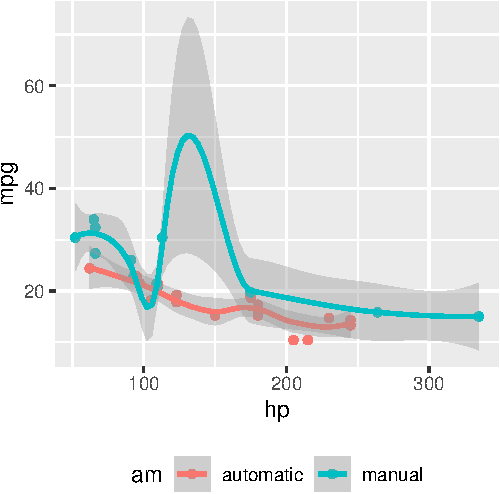
\includegraphics{tufte_template_files/figure-latex/fig-margin-1} 

}

\caption[MPG vs horsepower, colored by transmission]{MPG vs horsepower, colored by transmission.}\label{fig:fig-margin}
\end{marginfigure}

Note the use of the \texttt{fig.cap} chunk option to provide a figure
caption. You can adjust the proportions of figures using the
\texttt{fig.width} and \texttt{fig.height} chunk options. These are
specified in inches, and will be automatically scaled down to fit within
the handout margin.

\hypertarget{arbitrary-margin-content}{%
\subsection{Arbitrary Margin Content}\label{arbitrary-margin-content}}

In fact, you can include anything in the margin using the \textbf{knitr}
engine named \texttt{marginfigure}. Unlike R code chunks
\texttt{\textasciigrave{}\textasciigrave{}\textasciigrave{}\{r\}}, you
write a chunk starting with
\texttt{\textasciigrave{}\textasciigrave{}\textasciigrave{}\{marginfigure\}}
instead, then put the content in the chunk. See an example on the right
about the first fundamental theorem of calculus.

\begin{marginfigure}
We know from \emph{the first fundamental theorem of calculus} that for
\(x\) in \([a, b]\):
\[\frac{d}{dx}\left( \int_{a}^{x} f(u)\,du\right)=f(x).\]
\end{marginfigure}

For the sake of portability between LaTeX and HTML, you should keep the
margin content as simple as possible (syntax-wise) in the
\texttt{marginefigure} blocks. You may use simple Markdown syntax like
\texttt{**bold**} and \texttt{\_italic\_} text, but please refrain from
using footnotes, citations, or block-level elements (e.g.~blockquotes
and lists) there.

Note: if you set \texttt{echo\ =\ FALSE} in your global chunk options,
you will have to add \texttt{echo\ =\ TRUE} to the chunk to display a
margin figure, for example
\texttt{\textasciigrave{}\textasciigrave{}\textasciigrave{}\{marginfigure,\ echo\ =\ TRUE\}}.

\hypertarget{full-width-figures}{%
\subsection{Full Width Figures}\label{full-width-figures}}

You can arrange for figures to span across the entire page by using the
chunk option \texttt{fig.fullwidth\ =\ TRUE}.

\begin{Shaded}
\begin{Highlighting}[numbers=left,,]
\FunctionTok{ggplot}\NormalTok{(diamonds, }\FunctionTok{aes}\NormalTok{(carat, price)) }\SpecialCharTok{+} \FunctionTok{geom\_smooth}\NormalTok{() }\SpecialCharTok{+}
  \FunctionTok{facet\_grid}\NormalTok{(}\SpecialCharTok{\textasciitilde{}}\NormalTok{ cut)}
\end{Highlighting}
\end{Shaded}

\begin{figure*}

{\centering 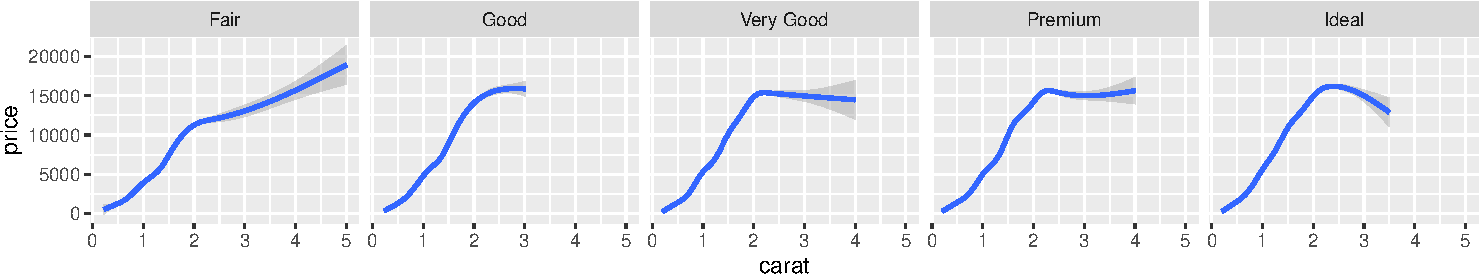
\includegraphics{tufte_template_files/figure-latex/fig-fullwidth-1} 

}

\caption[A full width figure]{A full width figure.}\label{fig:fig-fullwidth}
\end{figure*}

Other chunk options related to figures can still be used, such as
\texttt{fig.width}, \texttt{fig.cap}, \texttt{out.width}, and so on. For
full width figures, usually \texttt{fig.width} is large and
\texttt{fig.height} is small. In the above example, the plot size is
\(10 \times 2\).

\hypertarget{arbitrary-full-width-content}{%
\subsection{Arbitrary Full Width
Content}\label{arbitrary-full-width-content}}

Any content can span to the full width of the page. This feature
requires Pandoc 2.0 or above. All you need is to put your content in a
fenced \texttt{Div} with the class \texttt{fullwidth}, e.g.,

\begin{Shaded}
\begin{Highlighting}[]
\NormalTok{::: \{.fullwidth\}}
\NormalTok{Any \_full width\_ content here.}
\NormalTok{:::}
\end{Highlighting}
\end{Shaded}

Below is an example:

\emph{R is free software and comes with ABSOLUTELY NO WARRANTY.} You are
welcome to redistribute it under the terms of the GNU General Public
License versions 2 or 3. For more information about these matters see
\url{https://www.gnu.org/licenses/}.

\hypertarget{main-column-figures}{%
\subsection{Main Column Figures}\label{main-column-figures}}

Besides margin and full width figures, you can of course also include
figures constrained to the main column. This is the default type of
figures in the LaTeX/HTML output.

\begin{Shaded}
\begin{Highlighting}[numbers=left,,]
\FunctionTok{ggplot}\NormalTok{(diamonds, }\FunctionTok{aes}\NormalTok{(cut, price)) }\SpecialCharTok{+} \FunctionTok{geom\_boxplot}\NormalTok{()}
\end{Highlighting}
\end{Shaded}

\begin{figure}

{\centering 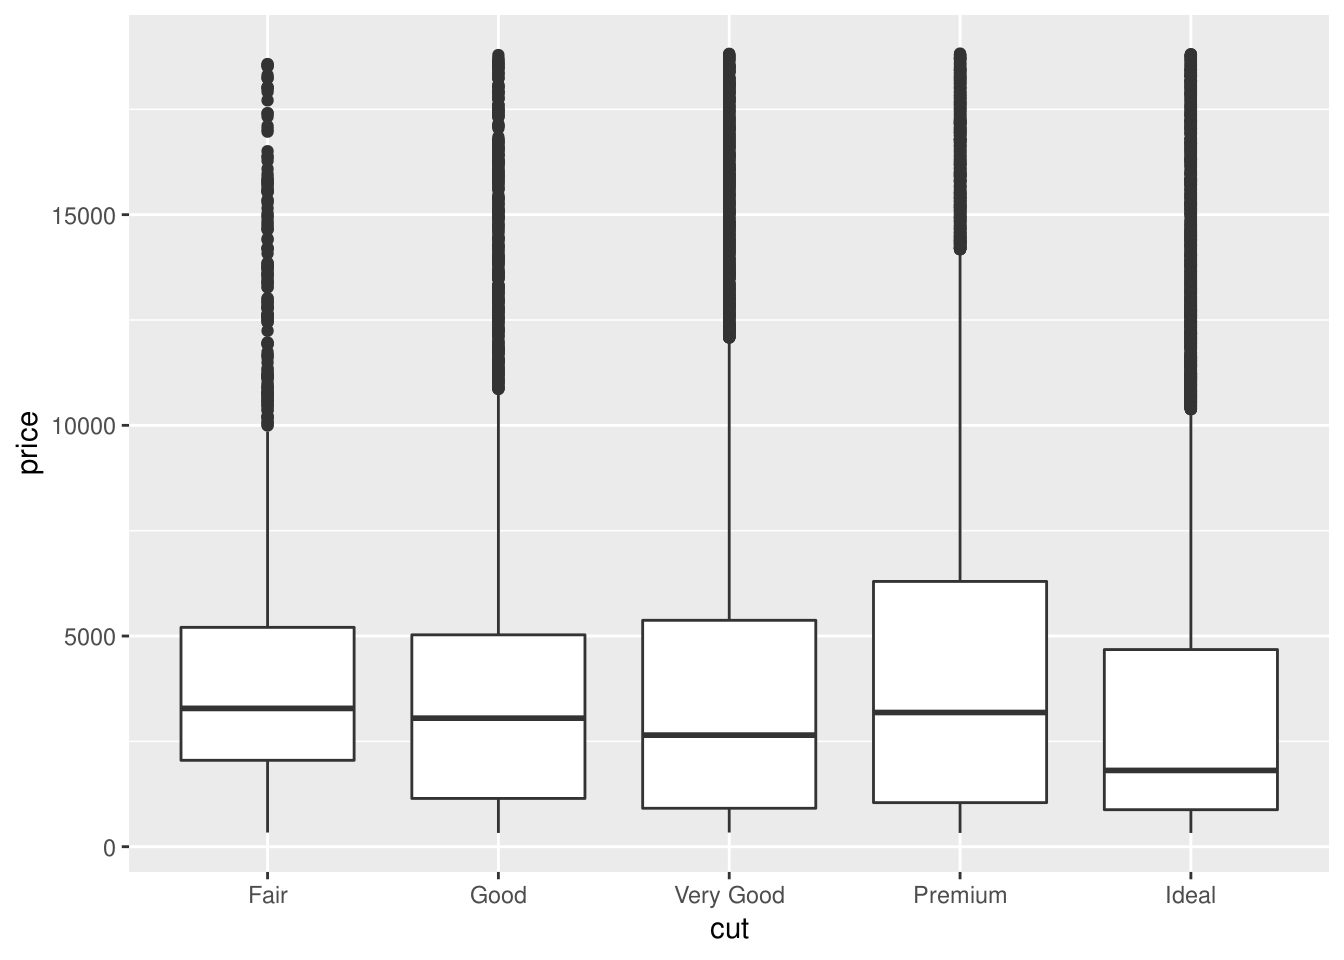
\includegraphics{tufte_template_files/figure-latex/fig-main-1} 

}

\caption[A figure in the main column]{A figure in the main column.}\label{fig:fig-main}
\end{figure}

\hypertarget{sidenotes}{%
\section{Sidenotes}\label{sidenotes}}

One of the most prominent and distinctive features of this style is the
extensive use of sidenotes. There is a wide margin to provide ample room
for sidenotes and small figures. Any use of a footnote will
automatically be converted to a sidenote. \footnote{This is a sidenote
  that was entered using a footnote.}

If you'd like to place ancillary information in the margin without the
sidenote mark (the superscript number), you can use the
\texttt{margin\_note()} function from \textbf{tufte} in an inline R
expression.
\marginnote{This is a margin note.  Notice that there is no number preceding the note.}
This function does not process the text with Pandoc, so Markdown syntax
will not work here. If you need to write anything in Markdown syntax,
please use the \texttt{marginfigure} block described previously.

\hypertarget{references}{%
\section{References}\label{references}}

References can be displayed as margin notes for HTML output. For
example, we can cite R here \citep{R-base}. To enable this feature, you
must set \texttt{link-citations:\ yes} in the YAML metadata, and the
version of \texttt{pandoc-citeproc} should be at least 0.7.2. You can
always install your own version of Pandoc from
\url{https://pandoc.org/installing.html} if the version is not
sufficient. To check the version of \texttt{pandoc-citeproc} in your
system, you may run this in R:

\begin{Shaded}
\begin{Highlighting}[numbers=left,,]
\FunctionTok{system2}\NormalTok{(}\StringTok{\textquotesingle{}pandoc{-}citeproc\textquotesingle{}}\NormalTok{, }\StringTok{\textquotesingle{}{-}{-}version\textquotesingle{}}\NormalTok{)}
\end{Highlighting}
\end{Shaded}

If your version of \texttt{pandoc-citeproc} is too low, or you did not
set \texttt{link-citations:\ yes} in YAML, references in the HTML output
will be placed at the end of the output document.

\hypertarget{tables}{%
\section{Tables}\label{tables}}

You can use the \texttt{kable()} function from the \textbf{knitr}
package to format tables that integrate well with the rest of the Tufte
handout style. The table captions are placed in the margin like figures
in the HTML output.

\begin{Shaded}
\begin{Highlighting}[numbers=left,,]
\NormalTok{knitr}\SpecialCharTok{::}\FunctionTok{kable}\NormalTok{(}
\NormalTok{  mtcars[}\DecValTok{1}\SpecialCharTok{:}\DecValTok{6}\NormalTok{, }\DecValTok{1}\SpecialCharTok{:}\DecValTok{6}\NormalTok{], }\AttributeTok{caption =} \StringTok{\textquotesingle{}A subset of mtcars.\textquotesingle{}}
\NormalTok{)}
\end{Highlighting}
\end{Shaded}

\begin{table}

\caption{\label{tab:unnamed-chunk-4}A subset of mtcars.}
\centering
\begin{tabular}[t]{l|r|r|r|r|r|r}
\hline
  & mpg & cyl & disp & hp & drat & wt\\
\hline
Mazda RX4 & 21.0 & 6 & 160 & 110 & 3.90 & 2.620\\
\hline
Mazda RX4 Wag & 21.0 & 6 & 160 & 110 & 3.90 & 2.875\\
\hline
Datsun 710 & 22.8 & 4 & 108 & 93 & 3.85 & 2.320\\
\hline
Hornet 4 Drive & 21.4 & 6 & 258 & 110 & 3.08 & 3.215\\
\hline
Hornet Sportabout & 18.7 & 8 & 360 & 175 & 3.15 & 3.440\\
\hline
Valiant & 18.1 & 6 & 225 & 105 & 2.76 & 3.460\\
\hline
\end{tabular}
\end{table}

\hypertarget{block-quotes}{%
\section{Block Quotes}\label{block-quotes}}

We know from the Markdown syntax that paragraphs that start with
\texttt{\textgreater{}} are converted to block quotes. If you want to
add a right-aligned footer for the quote, you may use the function
\texttt{quote\_footer()} from \textbf{tufte} in an inline R expression.
Here is an example:

\begin{quote}
``If it weren't for my lawyer, I'd still be in prison. It went a lot
faster with two people digging.''

\hfill --- Joe Martin
\end{quote}

Without using \texttt{quote\_footer()}, it looks like this (the second
line is just a normal paragraph):

\begin{quote}
``Great people talk about ideas, average people talk about things, and
small people talk about wine.''

--- Fran Lebowitz
\end{quote}

\hypertarget{responsiveness}{%
\section{Responsiveness}\label{responsiveness}}

The HTML page is responsive in the sense that when the page width is
smaller than 760px, sidenotes and margin notes will be hidden by
default. For sidenotes, you can click their numbers (the superscripts)
to toggle their visibility. For margin notes, you may click the circled
plus signs to toggle visibility.

\hypertarget{more-examples}{%
\section{More Examples}\label{more-examples}}

The rest of this document consists of a few test cases to make sure
everything still works well in slightly more complicated scenarios.
First we generate two plots in one figure environment with the chunk
option \texttt{fig.show\ =\ \textquotesingle{}hold\textquotesingle{}}:

\begin{Shaded}
\begin{Highlighting}[numbers=left,,]
\NormalTok{p }\OtherTok{\textless{}{-}} \FunctionTok{ggplot}\NormalTok{(mtcars2, }\FunctionTok{aes}\NormalTok{(hp, mpg, }\AttributeTok{color =}\NormalTok{ am)) }\SpecialCharTok{+}
  \FunctionTok{geom\_point}\NormalTok{()}
\NormalTok{p}
\NormalTok{p }\SpecialCharTok{+} \FunctionTok{geom\_smooth}\NormalTok{()}
\end{Highlighting}
\end{Shaded}

\begin{figure}

{\centering 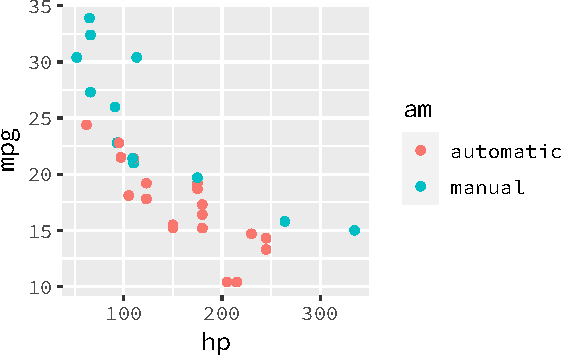
\includegraphics{tufte_template_files/figure-latex/fig-two-together-1} 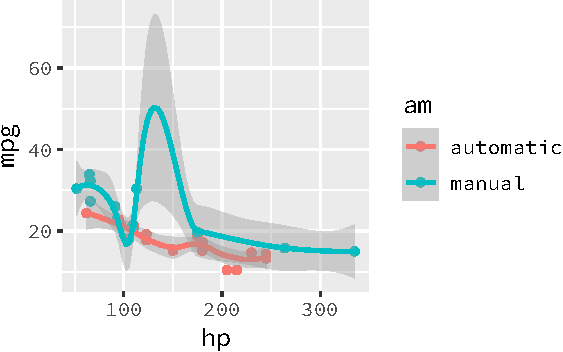
\includegraphics{tufte_template_files/figure-latex/fig-two-together-2} 

}

\caption[Two plots in one figure environment]{Two plots in one figure environment.}\label{fig:fig-two-together}
\end{figure}

Then two plots in separate figure environments (the code is identical to
the previous code chunk, but the chunk option is the default
\texttt{fig.show\ =\ \textquotesingle{}asis\textquotesingle{}} now):

\begin{Shaded}
\begin{Highlighting}[numbers=left,,]
\NormalTok{p }\OtherTok{\textless{}{-}} \FunctionTok{ggplot}\NormalTok{(mtcars2, }\FunctionTok{aes}\NormalTok{(hp, mpg, }\AttributeTok{color =}\NormalTok{ am)) }\SpecialCharTok{+}
  \FunctionTok{geom\_point}\NormalTok{()}
\NormalTok{p}
\end{Highlighting}
\end{Shaded}

\begin{figure}

{\centering 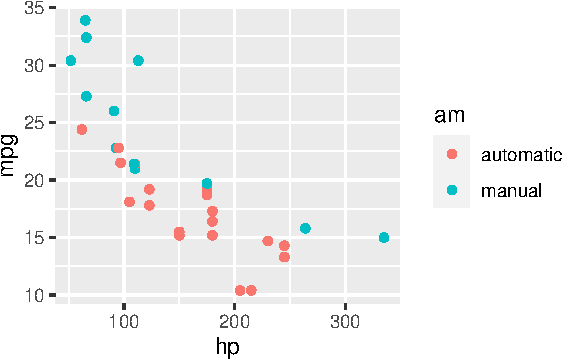
\includegraphics{tufte_template_files/figure-latex/fig-two-separate-1} 

}

\caption[Two plots in separate figure environments (the first plot)]{Two plots in separate figure environments (the first plot).}\label{fig:fig-two-separate-1}
\end{figure}

\begin{Shaded}
\begin{Highlighting}[numbers=left,,]
\NormalTok{p }\SpecialCharTok{+} \FunctionTok{geom\_smooth}\NormalTok{()}
\end{Highlighting}
\end{Shaded}

\begin{figure}

{\centering 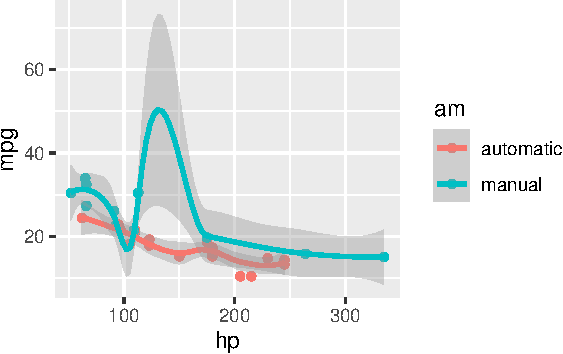
\includegraphics{tufte_template_files/figure-latex/fig-two-separate-2} 

}

\caption[Two plots in separate figure environments (the second plot)]{Two plots in separate figure environments (the second plot).}\label{fig:fig-two-separate-2}
\end{figure}

You may have noticed that the two figures have different captions, and
that is because we used a character vector of length 2 for the chunk
option \texttt{fig.cap} (something like
\texttt{fig.cap\ =\ c(\textquotesingle{}first\ plot\textquotesingle{},\ \textquotesingle{}second\ plot\textquotesingle{})}).

Next we show multiple plots in margin figures. Similarly, two plots in
the same figure environment in the margin:

\begin{Shaded}
\begin{Highlighting}[numbers=left,,]
\NormalTok{p}
\NormalTok{p }\SpecialCharTok{+} \FunctionTok{geom\_smooth}\NormalTok{(}\AttributeTok{method =} \StringTok{\textquotesingle{}lm\textquotesingle{}}\NormalTok{)}
\end{Highlighting}
\end{Shaded}

\begin{verbatim}
## `geom_smooth()` using formula 'y ~ x'
\end{verbatim}

\begin{marginfigure}

{\centering 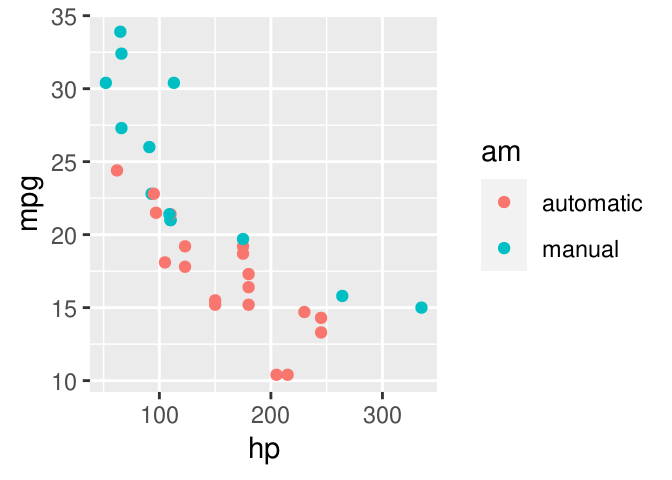
\includegraphics{tufte_template_files/figure-latex/fig-margin-together-1} 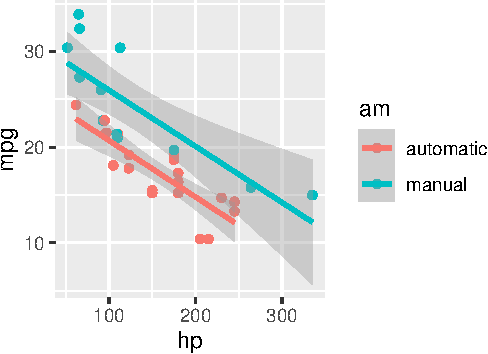
\includegraphics{tufte_template_files/figure-latex/fig-margin-together-2} 

}

\caption[Two plots in one figure environment in the margin]{Two plots in one figure environment in the margin.}\label{fig:fig-margin-together}
\end{marginfigure}

Then two plots from the same code chunk placed in different figure
environments:

\begin{Shaded}
\begin{Highlighting}[numbers=left,,]
\NormalTok{knitr}\SpecialCharTok{::}\FunctionTok{kable}\NormalTok{(}\FunctionTok{head}\NormalTok{(iris, }\DecValTok{15}\NormalTok{))}
\end{Highlighting}
\end{Shaded}

\begin{longtable}[]{@{}rrrrl@{}}
\toprule
Sepal.Length & Sepal.Width & Petal.Length & Petal.Width & Species \\
\midrule
\endhead
5.1 & 3.5 & 1.4 & 0.2 & setosa \\
4.9 & 3.0 & 1.4 & 0.2 & setosa \\
4.7 & 3.2 & 1.3 & 0.2 & setosa \\
4.6 & 3.1 & 1.5 & 0.2 & setosa \\
5.0 & 3.6 & 1.4 & 0.2 & setosa \\
5.4 & 3.9 & 1.7 & 0.4 & setosa \\
4.6 & 3.4 & 1.4 & 0.3 & setosa \\
5.0 & 3.4 & 1.5 & 0.2 & setosa \\
4.4 & 2.9 & 1.4 & 0.2 & setosa \\
4.9 & 3.1 & 1.5 & 0.1 & setosa \\
5.4 & 3.7 & 1.5 & 0.2 & setosa \\
4.8 & 3.4 & 1.6 & 0.2 & setosa \\
4.8 & 3.0 & 1.4 & 0.1 & setosa \\
4.3 & 3.0 & 1.1 & 0.1 & setosa \\
5.8 & 4.0 & 1.2 & 0.2 & setosa \\
\bottomrule
\end{longtable}

\begin{Shaded}
\begin{Highlighting}[numbers=left,,]
\NormalTok{p}
\end{Highlighting}
\end{Shaded}

\begin{marginfigure}

{\centering 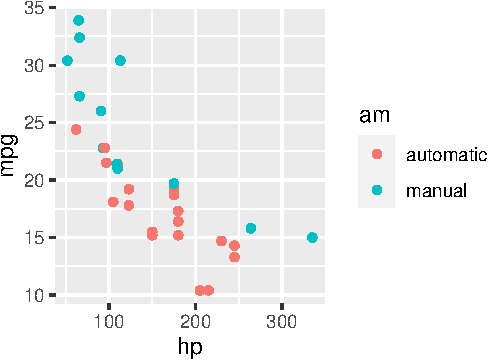
\includegraphics{tufte_template_files/figure-latex/fig-margin-separate-1} 

}

\caption[Two plots in separate figure environments in the margin (the first plot)]{Two plots in separate figure environments in the margin (the first plot).}\label{fig:fig-margin-separate-1}
\end{marginfigure}

\begin{Shaded}
\begin{Highlighting}[numbers=left,,]
\NormalTok{knitr}\SpecialCharTok{::}\FunctionTok{kable}\NormalTok{(}\FunctionTok{head}\NormalTok{(iris, }\DecValTok{12}\NormalTok{))}
\end{Highlighting}
\end{Shaded}

\begin{longtable}[]{@{}rrrrl@{}}
\toprule
Sepal.Length & Sepal.Width & Petal.Length & Petal.Width & Species \\
\midrule
\endhead
5.1 & 3.5 & 1.4 & 0.2 & setosa \\
4.9 & 3.0 & 1.4 & 0.2 & setosa \\
4.7 & 3.2 & 1.3 & 0.2 & setosa \\
4.6 & 3.1 & 1.5 & 0.2 & setosa \\
5.0 & 3.6 & 1.4 & 0.2 & setosa \\
5.4 & 3.9 & 1.7 & 0.4 & setosa \\
4.6 & 3.4 & 1.4 & 0.3 & setosa \\
5.0 & 3.4 & 1.5 & 0.2 & setosa \\
4.4 & 2.9 & 1.4 & 0.2 & setosa \\
4.9 & 3.1 & 1.5 & 0.1 & setosa \\
5.4 & 3.7 & 1.5 & 0.2 & setosa \\
4.8 & 3.4 & 1.6 & 0.2 & setosa \\
\bottomrule
\end{longtable}

\begin{Shaded}
\begin{Highlighting}[numbers=left,,]
\NormalTok{p }\SpecialCharTok{+} \FunctionTok{geom\_smooth}\NormalTok{(}\AttributeTok{method =} \StringTok{\textquotesingle{}lm\textquotesingle{}}\NormalTok{)}
\end{Highlighting}
\end{Shaded}

\begin{verbatim}
## `geom_smooth()` using formula 'y ~ x'
\end{verbatim}

\begin{marginfigure}

{\centering 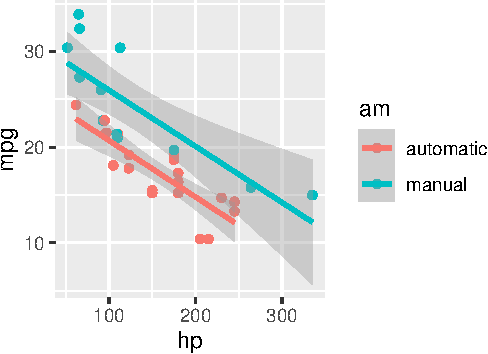
\includegraphics{tufte_template_files/figure-latex/fig-margin-separate-2} 

}

\caption[Two plots in separate figure environments in the margin (the second plot)]{Two plots in separate figure environments in the margin (the second plot).}\label{fig:fig-margin-separate-2}
\end{marginfigure}

\begin{Shaded}
\begin{Highlighting}[numbers=left,,]
\NormalTok{knitr}\SpecialCharTok{::}\FunctionTok{kable}\NormalTok{(}\FunctionTok{head}\NormalTok{(iris, }\DecValTok{5}\NormalTok{))}
\end{Highlighting}
\end{Shaded}

\begin{longtable}[]{@{}rrrrl@{}}
\toprule
Sepal.Length & Sepal.Width & Petal.Length & Petal.Width & Species \\
\midrule
\endhead
5.1 & 3.5 & 1.4 & 0.2 & setosa \\
4.9 & 3.0 & 1.4 & 0.2 & setosa \\
4.7 & 3.2 & 1.3 & 0.2 & setosa \\
4.6 & 3.1 & 1.5 & 0.2 & setosa \\
5.0 & 3.6 & 1.4 & 0.2 & setosa \\
\bottomrule
\end{longtable}

We blended some tables in the above code chunk only as
\emph{placeholders} to make sure there is enough vertical space among
the margin figures, otherwise they will be stacked tightly together. For
a practical document, you should not insert too many margin figures
consecutively and make the margin crowded.

You do not have to assign captions to figures. We show three figures
with no captions below in the margin, in the main column, and in full
width, respectively.

\begin{Shaded}
\begin{Highlighting}[numbers=left,,]
\CommentTok{\# a boxplot of weight vs transmission; this figure}
\CommentTok{\# will be placed in the margin}
\FunctionTok{ggplot}\NormalTok{(mtcars2, }\FunctionTok{aes}\NormalTok{(am, wt)) }\SpecialCharTok{+} \FunctionTok{geom\_boxplot}\NormalTok{() }\SpecialCharTok{+}
  \FunctionTok{coord\_flip}\NormalTok{()}
\end{Highlighting}
\end{Shaded}

\begin{marginfigure}

{\centering 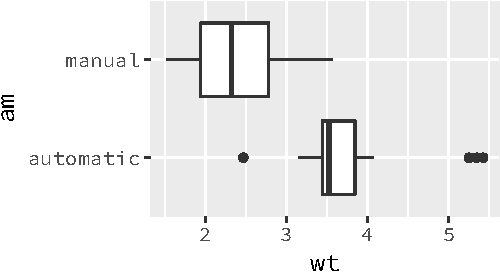
\includegraphics{tufte_template_files/figure-latex/fig-nocap-margin-1} 

}

\end{marginfigure}

\begin{Shaded}
\begin{Highlighting}[numbers=left,,]
\CommentTok{\# a figure in the main column}
\NormalTok{p }\OtherTok{\textless{}{-}} \FunctionTok{ggplot}\NormalTok{(mtcars, }\FunctionTok{aes}\NormalTok{(wt, hp)) }\SpecialCharTok{+} \FunctionTok{geom\_point}\NormalTok{()}
\NormalTok{p}
\end{Highlighting}
\end{Shaded}

\begin{center}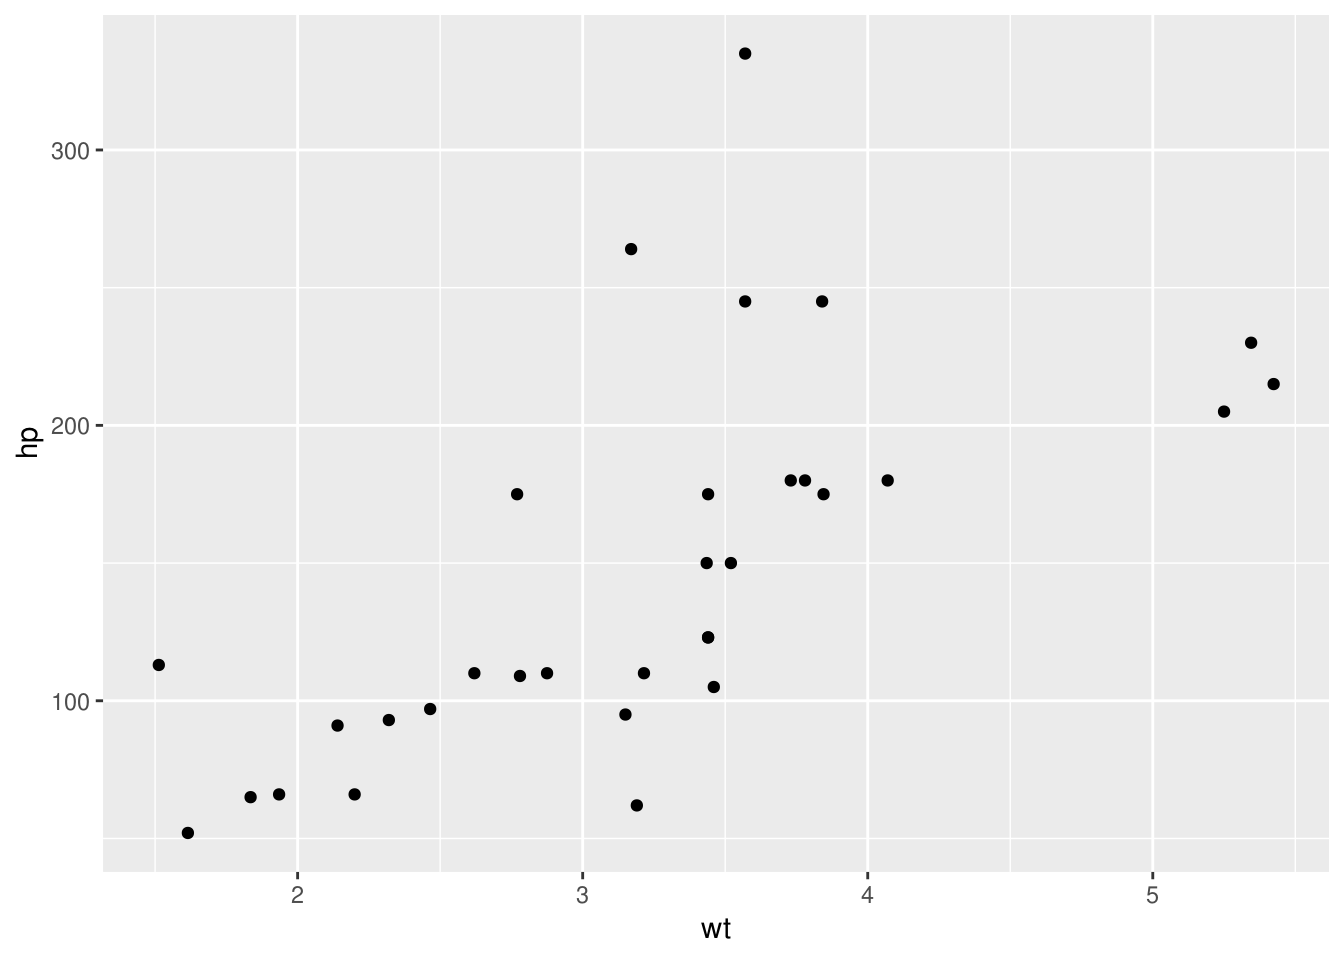
\includegraphics{tufte_template_files/figure-latex/fig-nocap-main-1} \end{center}

\begin{Shaded}
\begin{Highlighting}[numbers=left,,]
\CommentTok{\# a fullwidth figure}
\NormalTok{p }\SpecialCharTok{+} \FunctionTok{geom\_smooth}\NormalTok{(}\AttributeTok{method =} \StringTok{\textquotesingle{}lm\textquotesingle{}}\NormalTok{) }\SpecialCharTok{+} \FunctionTok{facet\_grid}\NormalTok{(}\SpecialCharTok{\textasciitilde{}}\NormalTok{ gear)}
\end{Highlighting}
\end{Shaded}

\begin{verbatim}
## `geom_smooth()` using formula 'y ~ x'
\end{verbatim}

\begin{figure*}

{\centering 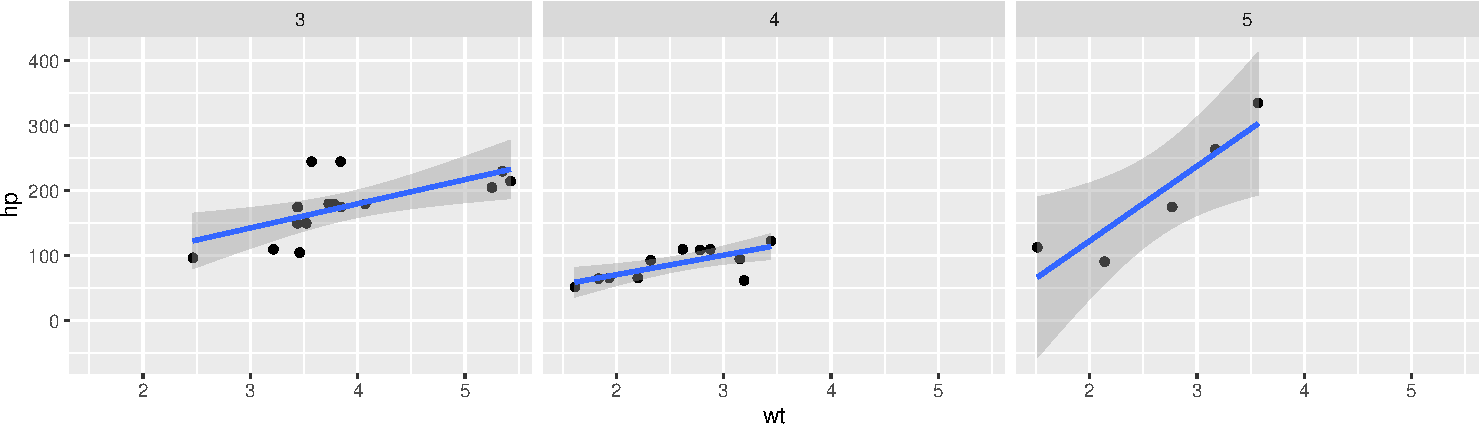
\includegraphics{tufte_template_files/figure-latex/fig-nocap-fullwidth-1} 

}

\end{figure*}

\hypertarget{some-notes-on-tufte-css}{%
\section{Some Notes on Tufte CSS}\label{some-notes-on-tufte-css}}

There are a few other things in Tufte CSS that we have not mentioned so
far. If you prefer \textsf{sans-serif fonts}, use the function
\texttt{sans\_serif()} in \textbf{tufte}. For epigraphs, you may use a
pair of underscores to make the paragraph italic in a block quote, e.g.

\begin{quote}
\emph{I can win an argument on any topic, against any opponent. People
know this, and steer clear of me at parties. Often, as a sign of their
great respect, they don't even invite me.}

\hfill --- Dave Barry
\end{quote}

We hope you will enjoy the simplicity of R Markdown and this R package,
and we sincerely thank the authors of the Tufte-CSS and Tufte-LaTeX
projects for developing the beautiful CSS and LaTeX classes. Our
\textbf{tufte} package would not have been possible without their heavy
lifting.

You can turn on/off some features of the Tufte style in HTML output. The
default features enabled are:

\begin{Shaded}
\begin{Highlighting}[]
\FunctionTok{output}\KeywordTok{:}
\AttributeTok{  tufte:}\FunctionTok{:tufte\_html}\KeywordTok{:}
\AttributeTok{    }\FunctionTok{tufte\_features}\KeywordTok{:}\AttributeTok{ }\KeywordTok{[}\StringTok{"fonts"}\KeywordTok{,}\AttributeTok{ }\StringTok{"background"}\KeywordTok{,}\AttributeTok{ }\StringTok{"italics"}\KeywordTok{]}
\end{Highlighting}
\end{Shaded}

If you do not want the page background to be lightyellow, you can remove
\texttt{background} from \texttt{tufte\_features}. You can also
customize the style of the HTML page via a CSS file. For example, if you
do not want the subtitle to be italic, you can define

\begin{Shaded}
\begin{Highlighting}[]
\NormalTok{h3}\FunctionTok{.subtitle}\NormalTok{ em \{}
  \KeywordTok{font{-}style}\NormalTok{: }\DecValTok{normal}\OperatorTok{;}
\NormalTok{\}}
\end{Highlighting}
\end{Shaded}

in, say, a CSS file \texttt{my\_style.css} (under the same directory of
your Rmd document), and apply it to your HTML output via the
\texttt{css} option, e.g.,

\begin{Shaded}
\begin{Highlighting}[]
\FunctionTok{output}\KeywordTok{:}
\AttributeTok{  tufte:}\FunctionTok{:tufte\_html}\KeywordTok{:}
\AttributeTok{    }\FunctionTok{tufte\_features}\KeywordTok{:}\AttributeTok{ }\KeywordTok{[}\StringTok{"fonts"}\KeywordTok{,}\AttributeTok{ }\StringTok{"background"}\KeywordTok{]}
\AttributeTok{    }\FunctionTok{css}\KeywordTok{:}\AttributeTok{ }\StringTok{"my\_style.css"}
\end{Highlighting}
\end{Shaded}

There is also a variant of the Tufte style in HTML/CSS named
``\href{https://github.com/nogginfuel/envisioned-css}{Envisoned CSS}''.
This style can be used by specifying the argument
\texttt{tufte\_variant\ =\ \textquotesingle{}envisioned\textquotesingle{}}
in \texttt{tufte\_html()}\footnote{The actual Envisioned CSS was not
  used in the \textbf{tufte} package. We only changed the fonts,
  background color, and text color based on the default Tufte style.},
e.g.

\begin{Shaded}
\begin{Highlighting}[]
\FunctionTok{output}\KeywordTok{:}
\AttributeTok{  tufte:}\FunctionTok{:tufte\_html}\KeywordTok{:}
\AttributeTok{    }\FunctionTok{tufte\_variant}\KeywordTok{:}\AttributeTok{ }\StringTok{"envisioned"}
\end{Highlighting}
\end{Shaded}

To see the R Markdown source of this example document, you may follow
\href{https://github.com/rstudio/tufte/raw/master/inst/rmarkdown/templates/tufte_html/skeleton/skeleton.Rmd}{this
link to Github}, use the wizard in RStudio IDE
(\texttt{File\ -\textgreater{}\ New\ File\ -\textgreater{}\ R\ Markdown\ -\textgreater{}\ From\ Template}),
or open the Rmd file in the package:

\begin{Shaded}
\begin{Highlighting}[numbers=left,,]
\FunctionTok{file.edit}\NormalTok{(}
\NormalTok{  tufte}\SpecialCharTok{:::}\FunctionTok{template\_resources}\NormalTok{(}
    \StringTok{\textquotesingle{}tufte\_html\textquotesingle{}}\NormalTok{, }\StringTok{\textquotesingle{}..\textquotesingle{}}\NormalTok{, }\StringTok{\textquotesingle{}skeleton\textquotesingle{}}\NormalTok{, }\StringTok{\textquotesingle{}skeleton.Rmd\textquotesingle{}}
\NormalTok{  )}
\NormalTok{)}
\end{Highlighting}
\end{Shaded}

This document is also available in
\href{https://rstudio.github.io/tufte/cn/}{Chinese}, and its
\texttt{envisioned} style can be found
\href{https://rstudio.github.io/tufte/envisioned/}{here}.

\bibliography{./bib/skeleton.bib}



\end{document}
